\chapter{Data and Materials}
\label{chapter:materials}

\begin{introduction}
\begin{flushright}
``They're business expenses.''
\end{flushright}

\vspace{0.5em}

This chapter describes the financial instruments and data sources that form the empirical foundation of the study. It motivates the choice of GICS-based sector ETFs as the investment universe, then details the collection and preprocessing of two complementary textual streams: financial news from the GDELT Project and social media discussions from Reddit.
\end{introduction}

This chapter describes the financial instruments and datasets that form the empirical foundation of this study. Portfolio optimization requires a clearly defined investment universe, and the selection of appropriate data sources is therefore essential for constructing reliable and reproducible results, and for testing the hypotheses outlined in Section~\ref{sec:sota_hypothesis}. Three data streams are employed: sector-based ETF market data (Section~\ref{sec:etfs}), financial news (Section~\ref{sec:gdelt}), and social media content (Section~\ref{sec:reddit}).

Beyond market data, the inclusion of textual sources alongside market prices is motivated by the distinct and complementary informational roles hypothesized for news and social media. These two streams are expected to reflect both information-driven views and fast-moving market reactions \cite{9d5c9}, enabling the empirical evaluation of a dual-layer sentiment structure and its relative contribution to sector-level return predictions.


\section{Sector-Based ETFs}
\label{sec:etfs}

Sector-based portfolio construction requires a principled taxonomy to partition the investment universe into economically meaningful and mutually exclusive groups. Without a standardized classification framework, sector boundaries become arbitrary, making it difficult to ensure clean return attribution, reproduce results across studies, or align the portfolio with widely used benchmarks.

Several such frameworks exist, each offering a structured approach to classifying companies by their primary business activities. Notable examples include the Industry Classification Benchmark (ICB), maintained by FTSE Russell, and the Thomson Reuters Business Classification (TRBC). Despite these alternatives, the Global Industry Classification Standard (GICS), developed jointly by S\&P Dow Jones Indices and Morgan Stanley Capital International (MSCI) in 1999, has emerged as the dominant framework. Its widespread adoption in both academic research and professional investment practice reflects its consistency, transparency, and close alignment with major equity benchmarks \cite{fefa8, 781c5}.

\subsection{The GICS Framework}
\label{subsec:gics}

GICS offers a coherent and transparent framework for systematically categorizing companies across global equity markets. It employs a four-tier hierarchical structure, comprising 11 sectors, 25 industry groups, 74 industries, and 163 sub-industries (Fig.~\ref{fig:gics_sectors_diagram}), facilitating detailed and scalable analysis. By assigning firms based on their primary business activities, GICS supports a wide range of applications, including investment research, portfolio construction, and strategic asset allocation \cite{c5103}.

\begin{figure}[ht]
    \centering
    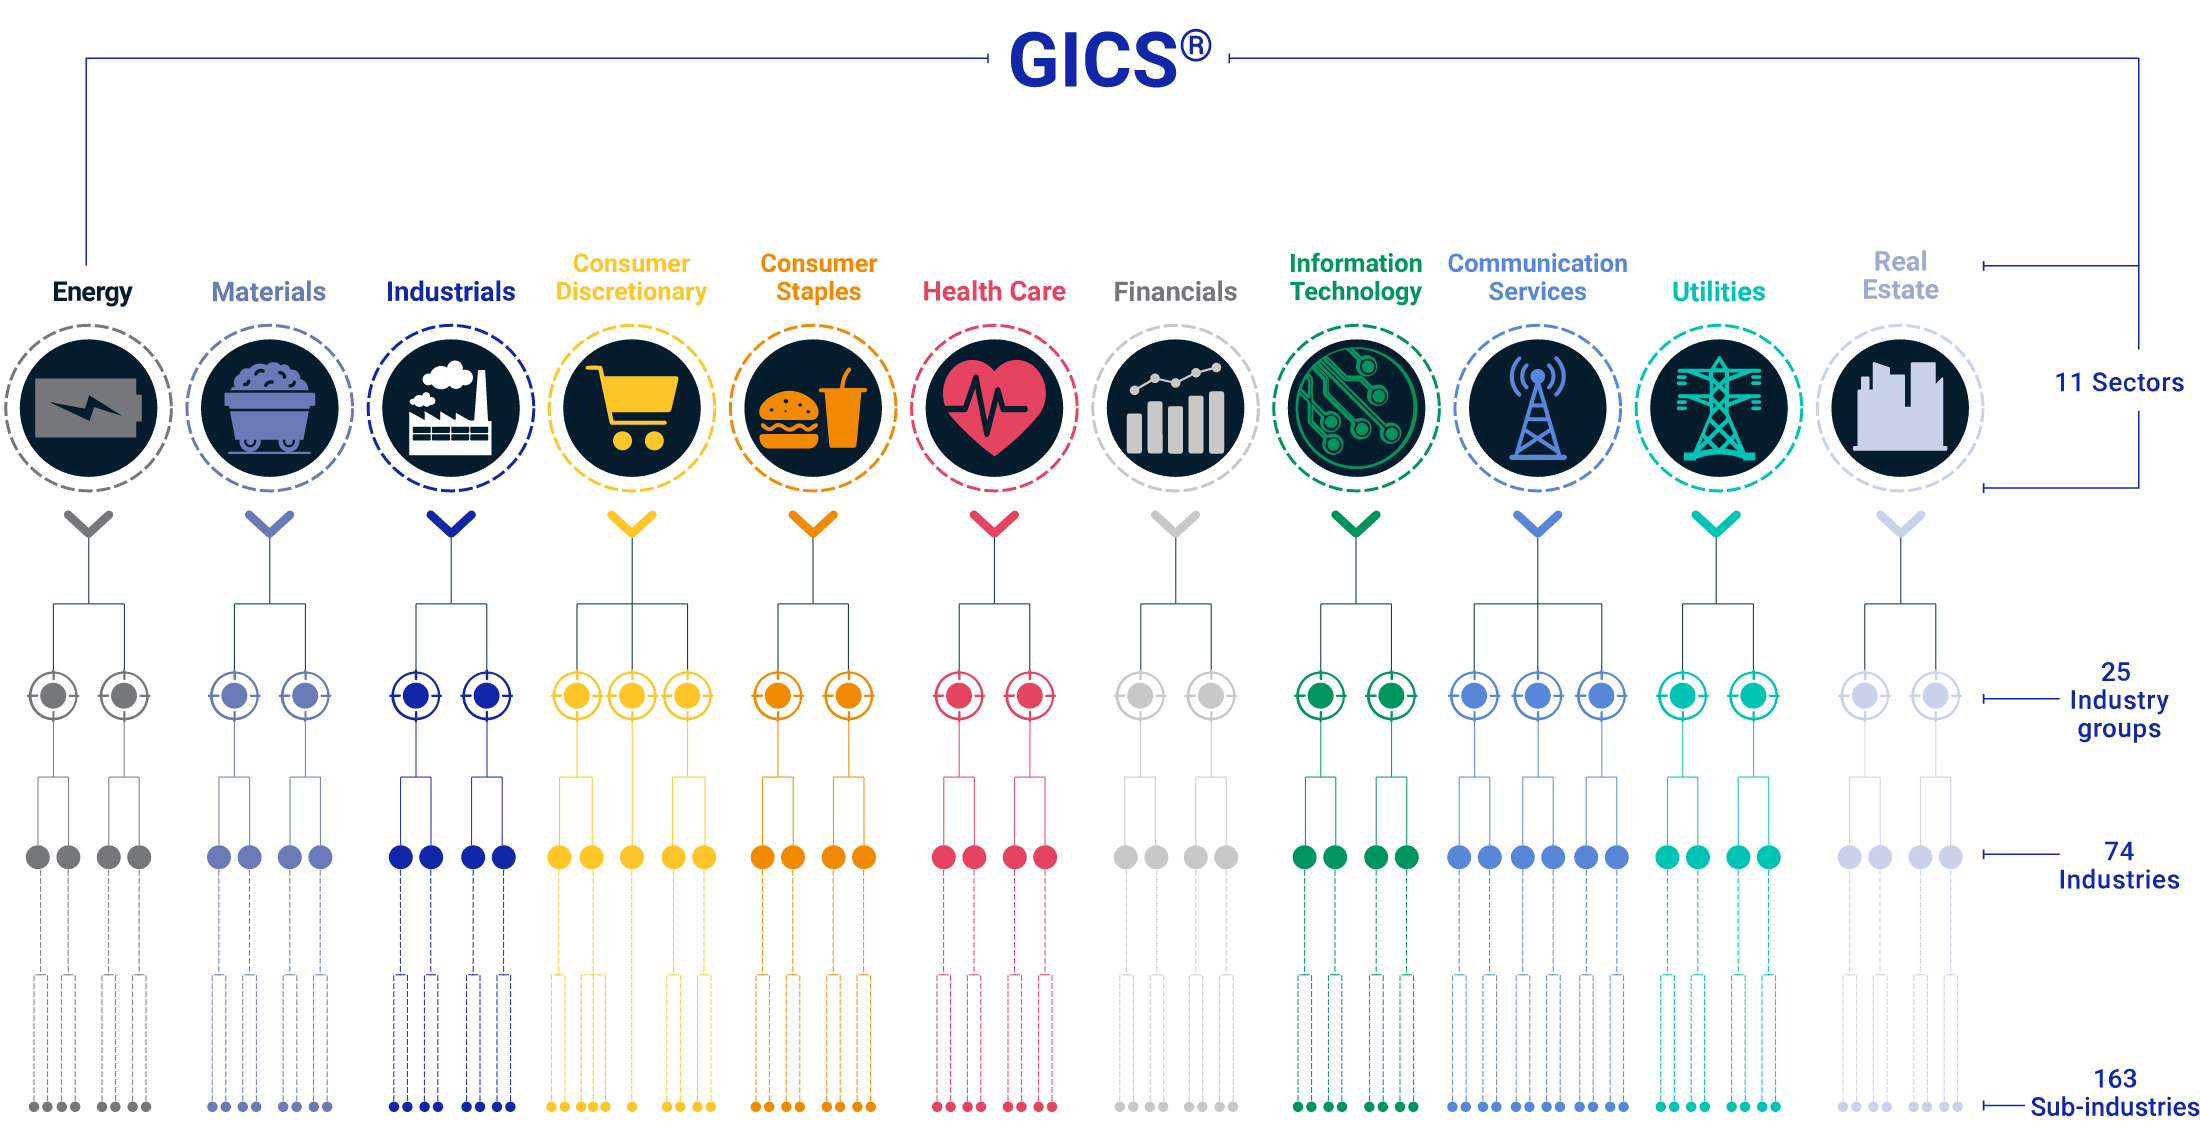
\includegraphics[width=1\textwidth]{figs/gics_sectors_infographic.png}
    \caption{The GICS hierarchical structure, illustrating the 11 sectors and their corresponding industry groups, industries, and sub-industries. Source: MSCI (\url{https://www.msci.com/indexes/index-resources/gics}).}
    \label{fig:gics_sectors_diagram}
\end{figure}

Its widespread adoption is largely driven by its integration with major benchmark providers, particularly S\&P Dow Jones Indices and MSCI, as well as the broad ecosystem of investable products built around it, such as sector-based ETFs. Combined with strong empirical support in the academic literature \cite{558b2}, these features make GICS a well-justified and methodologically robust foundation for portfolio construction in this study.

\subsection{Data Collection}
\label{subsec:etf_data}

The selection of the representative ETFs follows both practical investment considerations and methodological requirements. In real-world portfolio construction, essential criteria typically include high liquidity, low expense ratios, an established performance record, and a substantial asset base \cite{hill2015etf}. For the purposes of this research, two additional criteria were considered: the selected ETFs should allow for straightforward benchmarking against existing literature and real-world market performance, and they must provide sector-specific exposure with minimal overlap between sectors, ensuring clean attribution of returns and risk at the sector level.

Based on these requirements, the Select Sector SPDR ETFs series\footnote{\url{https://www.sectorspdrs.com}} was chosen, comprising 11 ETFs each tracking a specific GICS sector within the (Standard \& Poor's 500 Index) S\&P~500 Index. All funds are series of the Select Sector SPDR Trust, managed by State Street Global Advisors, ensuring operational consistency across the portfolio. The non-overlapping sector construction supports straightforward implementation of sector rotation, hedging, and tactical allocation strategies, and facilitates direct comparison with existing studies. Although reliance on a single fund provider could in principle introduce concentration risk, this consideration is set aside in the present study. The 11 ETFs are listed in Table~\ref{tab:sector_etfs}.

% \begin{table}[ht]
% \centering
% \caption{Overview of the Select Sector SPDR ETFs included in this study, detailing each ETF's corresponding GICS sector, ticker symbol, ISIN with reference sources, and inception date.}
% \label{tab:sector_etfs}
% \begin{tabular}{|l|c|l|c|}
% \hline
% \textbf{Sector} & \textbf{Ticker} & \textbf{ISIN / Links} & \textbf{Inception Date} \\
% \hline
% Energy & XLE & US81369Y5069 (\href{https://www.ssga.com/us/en/intermediary/etfs/the-energy-select-sector-spdr-fund-xle}{SSGA}, \href{https://cbonds.com/etf/87/}{Cbonds}) & 1998-12-16 \\
% Materials & XLB & US81369Y1001 (\href{https://www.ssga.com/nl/en_gb/intermediary/etfs/the-materials-select-sector-spdr-fund-xlb}{SSGA}, \href{https://cbonds.com/etf/273/}{Cbonds}) & 1998-12-16 \\
% Industrials & XLI & US81369Y7040 (\href{https://www.ssga.com/se/en_gb/intermediary/etfs/the-industrial-select-sector-spdr-fund-xli}{SSGA}, \href{https://cbonds.com/etf/91/}{Cbonds}) & 1998-12-16 \\
% Consumer Discretionary & XLY & US81369Y4070 (\href{https://www.ssga.com/us/en/intermediary/etfs/the-consumer-discretionary-select-sector-spdr-fund-xly}{SSGA}, \href{https://cbonds.com/etf/79/}{Cbonds}) & 1998-12-16 \\
% Consumer Staples & XLP & US81369Y3080 (\href{https://www.ssga.com/us/en/intermediary/etfs/the-consumer-staples-select-sector-spdr-fund-xlp}{SSGA}, \href{https://cbonds.com/etf/81/}{Cbonds}) & 1998-12-16 \\
% Health Care & XLV & US81369Y2090 (\href{https://www.ssga.com/us/en/intermediary/etfs/the-health-care-select-sector-spdr-fund-xlv}{SSGA}, \href{https://cbonds.com/etf/89/}{Cbonds}) & 1998-12-16 \\
% Financials & XLF & US81369Y6059 (\href{https://www.ssga.com/us/en/intermediary/etfs/the-financial-select-sector-spdr-fund-xlf}{SSGA}, \href{https://cbonds.com/etf/1/}{Cbonds}) & 1998-12-16 \\
% Information Technology & XLK & US81369Y8030 (\href{https://www.ssga.com/us/en/intermediary/etfs/the-technology-select-sector-spdr-fund-xlk}{SSGA}, \href{https://cbonds.com/etf/21/}{Cbonds}) & 1998-12-16 \\
% Communication Services & XLC & US81369Y8527 (\href{https://www.ssga.com/us/en/intermediary/etfs/the-communication-services-select-sector-spdr-fund-xlc}{SSGA}, \href{https://cbonds.com/etf/2271/}{Cbonds}) & 2018-06-18 \\
% Utilities & XLU & US81369Y8865 (\href{https://www.ssga.com/us/en/intermediary/etfs/the-utilities-select-sector-spdr-fund-xlu}{SSGA}, \href{https://cbonds.com/etf/111/}{Cbonds}) & 1998-12-16 \\
% Real Estate & XLRE & US81369Y8600 (\href{https://www.ssga.com/us/en/intermediary/etfs/the-real-estate-select-sector-spdr-fund-xlre}{SSGA}, \href{https://cbonds.com/etf/2273/}{Cbonds}) & 2015-10-07 \\
% \hline
% \end{tabular}
% \caption*{\footnotesize
% Note: The SSGA (\url{https://www.ssga.com/}) and Cbonds (\url{https://cbonds.com/}) websites were used as data sources for the verification of ISIN codes and inception dates of each sector ETF.
% }
% \end{table}

\begin{table}[ht]
\centering
\caption{Overview of the Select Sector SPDR ETFs included in this study, detailing each ETF's corresponding GICS sector, ticker symbol, International Securities Identification Number (ISIN), and inception date.}
\label{tab:sector_etfs}
\begin{tabular}{|l|c|c|c|}
\hline
\textbf{Sector} & \textbf{Ticker} & \textbf{ISIN} & \textbf{Inception Date} \\
\hline
Energy                  & XLE   & US81369Y5069 & 1998-12-16 \\
Materials               & XLB   & US81369Y1001 & 1998-12-16 \\
Industrials             & XLI   & US81369Y7040 & 1998-12-16 \\
Consumer Discretionary  & XLY   & US81369Y4070 & 1998-12-16 \\
Consumer Staples        & XLP   & US81369Y3080 & 1998-12-16 \\
Health Care             & XLV   & US81369Y2090 & 1998-12-16 \\
Financials              & XLF   & US81369Y6059 & 1998-12-16 \\
Information Technology  & XLK   & US81369Y8030 & 1998-12-16 \\
Communication Services  & XLC   & US81369Y8527 & 2018-06-18 \\
Utilities               & XLU   & US81369Y8865 & 1998-12-16 \\
Real Estate             & XLRE  & US81369Y8600 & 2015-10-07 \\
\hline
\end{tabular}
\caption*{\footnotesize
Note: The SSGA (\url{https://www.ssga.com/}) and Cbonds (\url{https://cbonds.com/}) websites were used as data sources for the verification of ISIN codes and inception dates of each sector ETF.
}
\end{table}


Market data were collected using \texttt{yfinance}\footnote{\url{https://pypi.org/project/yfinance}}, an open-source Python library providing programmatic access to historical financial data through Yahoo!\ Finance\footnote{\url{https://finance.yahoo.com/markets}}. \texttt{yfinance} is widely adopted in the academic literature for financial data collection \cite{e6ca3, 93d76, b58bb}, offering free and programmatic access to a broad range of instruments with extensive historical depth, making it well-suited for large-scale reproducible research. Daily data were collected over a ten-year horizon spanning July 1, 2015 to June 30, 2025. Two ETFs have inception dates falling within this window, namely XLRE and XLC, and for these, only data from their respective inception dates onward were used.

The raw dataset includes Open, High, Low, Close, Adjusted Close, Volume, Dividends, and Stock Splits for each ETF. To account for corporate actions such as dividends and stock splits, adjusted prices are used throughout the analysis rather than raw closing prices. The adjustment factor $A_{t}$ is computed as the ratio of the Adjusted Close to the raw Close provided by \texttt{yfinance}, at time $t$, and applied uniformly to the Open, High, and Low fields, ensuring consistency across all price series. This ensures consistency across all price series by placing them on a common adjusted basis. This approach simplifies implementation while preserving the cumulative impact of corporate actions on historical price movements.

Finally, the bid-ask spread was extracted. It serves as a standard proxy for the transaction  costs incurred when executing trades \cite{hill2015etf, bidask09}, and is incorporated into the portfolio optimization as a one-way cost applied proportionally to turnover at each rebalancing date. As no historical bid-ask spread data were found for the selected ETFs, the 30-day median bid-ask spread reported by State Street Global Advisors\footnote{\url{https://www.ssga.com}} was used as a fixed estimate, extracted on February 7, 2026. While this approach does not capture temporal variation in transaction costs, it provides a reasonable and consistent approximation given the typically stable and narrow spreads of large, liquid ETFs. The extracted spreads range from 0.01\% to 0.02\% across all 11 ETFs, reflecting the high liquidity characteristic of large-cap index funds.



\section{Financial News}
\label{sec:gdelt}

After evaluating several news data providers, such as ProQuest\footnote{\url{https://www.proquest.com}}, Bloomberg\footnote{\url{https://www.bloomberg.com}}, The New York Times\footnote{\url{https://www.nytimes.com}}, and Reuters\footnote{\url{https://www.reuters.com}}, the GDELT Project\footnote{\url{https://www.gdeltproject.org}} was selected as the primary source of financial news for this study. This decision was driven by the need for a large, reproducible corpus of news articles that could be programmatically accessed and processed at scale, which was not feasible with the evaluated providers due to practical limitations such as paywalls, restrictive licenses, API usage caps, and limited historical depth.

\subsection{The GDELT Project}
\label{subsec:gdelt_why}

The Global Database of Events, Language, and Tone (GDELT) Project, supported by Google Jigsaw, consists of a continuously updated database monitoring broadcast, print, and online news media, transforming articles into structured, machine-readable records. This study uses the GDELT 2.0 Global Knowledge Graph (GKG 2.0), which provides rich metadata including timestamps, source URLs, geographic information, themes, named entities, tone measures, and extracted quotations. These structured fields enable the transformation of unstructured news into quantitative features suitable for NLP pipelines. Beyond accessibility, GDELT offers strong historical coverage, consistent high-frequency updates, and broad geographic scope, with substantial coverage of U.S. sources that is particularly relevant given the central role of U.S. equity markets in this study~\cite{gdelt2015globalworld}.

It is worth noting that GDELT does not provide full article text, as the GKG automatically extracts discrete quotations identified within each monitored source. These quotations represent verbatim excerpts of relevant statements and are used in this study as a proxy for the informational content of the underlying news articles.

These characteristics make GDELT a well-suited choice for constructing a large-scale, reproducible dataset, enabling the empirical evaluation of news-based sentiment measures and their relationship with sector-level returns. Although GDELT's coverage is neither financial nor business-specific, this limitation is mitigated by the application of sector-specific filtering techniques, as described in the next section. This represents a necessary trade-off between domain specificity and the scalability and reproducibility requirements of this study.

\subsection{Data Collection}
\label{subsec:gdelt_data}

Historical GDELT data, from the GKG 2.0 dataset, were obtained from the public GDELT archive\footnote{\url{http://data.gdeltproject.org/gdeltv2/masterfilelist.txt}}, which distributes data as time-stamped compressed files at 15-minute intervals. All GKG files spanning July 1, 2015 to June 30, 2025 were programmatically accessed via a streaming, request-based pipeline, enabling large-scale historical collection while preserving full reproducibility. Each file consists of compressed tab-separated records which, after decompression, are parsed into structured dataframes. To reduce dimensionality, the dataset was restricted to four fields: the unique record identifier (\texttt{GKGRECORDID}), publication date, source name (\texttt{SourceCommonName}), and the quotations field. The themes and tone variables were excluded, as their classification relies on a proprietary and non-transparent taxonomy, thereby compromising methodological transparency.

As mentioned, GDELT's broad coverage necessitates a filtering step to isolate news relevant to each GICS sector. The ideal approach would involve leveraging the structured metadata fields, such as themes or named entities, to identify sector-specific content. However, these fields are not designed for financial classification and often lack the granularity or consistency required for accurate sector attribution. Instead, a term-based filtering approach was adopted, using sector-specific dictionaries to identify relevant news items based on the presence of key terms in the quotations field. Two candidate dictionaries were evaluated for this purpose.

The first dictionary was derived from TF-IDF\footnote{TF-IDF (Term Frequency-Inverse Document Frequency) is a text analysis statistic that scores words by how frequently they appear in a given document relative to how frequently they appear across the entire corpus, thus highlighting terms that are distinctive to specific documents or groups.} scores computed on 10-K filings of S\&P~500 firms grouped by sector, but the extracted terms were often overly specific, including company names and branded products, limiting generalizability. The second dictionary was generated using large language models (LLMs) (\texttt{meta-llama/Llama-3.1-8B-Instruct}, \texttt{google/gemma-7b-it}, and \texttt{Qwen/Qwen2.5-7B-Instruct}), which were each prompted with all 163 GICS sub-industry descriptions\footnote{\url{https://www.msci.com/documents/1296102/29559863/GICS_structure_and_definitions_effective_close_of_March_17_2023.xlsx}} to produce up to 10 representative terms per sub-industry. The resulting terms were lemmatized, assigned to their corresponding GICS sector based on the sub-industry they were generated from, and the most frequent lemmas per sector were retained. The LLM-based dictionary was selected for the final analysis as it yielded semantically representative yet sufficiently general terminology, avoiding firm-specific bias. The dictionary was truncated to 30 lemmas per sector based on the empirical frequency distribution, meaning that a quote is attributed to a sector if any of its top-30 lemmas appear in the quote's lemmatized tokens. The final filtering terms are reported in Table~\ref{tab:per_sector_filter_words}.

An additional source-level filtering step was then applied to reduce data volume and limit noise from non-essential outlets. First, only U.S.-based outlets were retained, identified via the GDELT Geographic Source Lookup\footnote{\url{https://blog.gdeltproject.org/mapping-the-media-a-geographic-lookup-of-gdelts-sources}}, ensuring geographic consistency with the U.S. equity universe. Within each sector, sources were ranked by their contribution to sector-specific coverage, approximated via frequency counts on a random 10\% sample of the data. Sources were then selected greedily, per sector, in descending order of volume until their cumulative contribution reached 10\% of total sector-related coverage, effectively capturing the small set of high-frequency outlets that dominate each sector's news flow. This threshold was determined empirically, balancing coverage reduction against representativeness while avoiding the story duplication and noise typical of lower-frequency outlets. The resulting source lists are reported in Table~\ref{tab:per_sector_filter_sources}.

After applying all filtering steps, the final dataset comprises $\num{8602613}$ news quotations spanning the full ten-year study period. This represents a substantial reduction from the raw archive, achieved through the combined term- and source-based filtering steps, while retaining a large and representative corpus of sector-relevant content for subsequent analysis.


\section{Social Media}
\label{sec:reddit}

Among the social media platforms most referenced in the academic literature for financial sentiment analysis, namely X\footnote{\url{https://x.com}} (formerly Twitter), StockTwits\footnote{\url{https://stocktwits.com}}, and Reddit\footnote{\url{https://www.reddit.com}}, Reddit was selected as the sole source for this study. Despite its large user base, X presents substantial challenges: its heterogeneous content makes sector-level segmentation difficult, and most academic studies employing it focus on individual firms or aggregate market sentiment rather than the sector-level dynamics required here. StockTwits, while explicitly finance-oriented and well-suited to asset-specific tagging, imposes significant data accessibility constraints, and as of December 2025, comprehensive historical access requires enterprise-level tools, creating practical barriers to reproducible research.

\subsection{Reddit as a Financial Data Source}
\label{subsec:reddit_why}

Reddit is structured around topic-focused communities called subreddits, which enable targeted data collection and support the construction of sector-relevant sentiment measures without relying on proprietary access arrangements. Given its large and active user base, Reddit's community-driven structure allows for the collection of both submissions (posts) and comments, providing a comprehensive view of user sentiment and engagement. Additionally, discussions often reflect collective sentiment and can capture emerging trends or shifts in market perception more rapidly than traditional news sources.

Three subreddits were selected for data collection, based on their substantial user engagement, thematic focus on equity markets, and their prevalence in existing financial sentiment research~\cite{da676, 5530e, cc28c}: \texttt{r/stocks}, \texttt{r/wallstreetbets}, and \texttt{r/investing}. Each has a distinct character: \texttt{r/investing} focuses on long-term, traditional investment strategies, \texttt{r/stocks} serves as a general forum for stock discussion and market news, and \texttt{r/wallstreetbets} is known for high-risk, speculative trading discussions. Collectively, they provide a diverse and representative sample of retail investor sentiment expressed on Reddit.

\subsection{Data Collection}
\label{subsec:reddit_data}

Data were collected spanning July 1, 2015 to June 30, 2025, consistent with the study period defined for the ETF and GDELT datasets. Among the extraction approaches evaluated (web scraping, the official Reddit API, and Pushshift), web scraping was deemed unsuitable due to scalability limitations and potential terms-of-service violations, while the official Reddit API imposes strict rate limits and provides limited historical depth, making Pushshift the most viable option for large-scale historical data collection.

Pushshift is a comprehensive archival resource for Reddit data offering extensive historical coverage and wide adoption in academic research. Since August 2023, however, direct API access has been restricted to approved moderation use cases~\cite{RedditPushshift2023}. This study therefore used a Pushshift data dump distributed via Academic Torrents\footnote{\url{https://academictorrents.com/details/30dee5f0406da7a353aff6a8caa2d54fd01f2ca1}} containing all publicly available Reddit submissions and comments from June 2005 to June 2025, totaling approximately \SI{3.46}{\tera\byte}. Given this scale, files were processed via a streaming pipeline, read line by line rather than loaded into memory, enabling efficient memory utilization and parallel processing.

The dataset was subsequently filtered to retain only content from the three target subreddits and within the study period. Low-engagement posts (scores of one or below) were removed to reduce noise. Comments were merged with their parent submissions to preserve conversational context, redundant fields were discarded to optimize storage, and submissions lacking textual content, such as image-only or video-only posts, were excluded from the analysis. After filtering, the final dataset comprises $\num{355352}$ posts spanning the full study period.